\section{Pozíció szabályozás állapotvisszacsatolással}

%{{{ Pólusok számítása
\subsection{Pólusok számítása}

\begin{figure}[H]
    \centering
	\incfig[\textwidth]{6a_allapotter_hatasvazlat_jav}
	\caption{Integrátorral kiegészített állapottér modell}
	\label{fig:6a_allapotter_hatasvazlat_jav}
\end{figure}

% \begin{equation}
%     \mat{\dot{x}_1\\\dot{x}_2\\ \dot{x}_\text{I}} =
%     \mat{0&0&0\\-5\cdot10^5&-7302&0\\-1&-1&0}\mat{x_1\\x_2\\x_\text{I}} +
%     \mat{0\\1\\0}u
% \end{equation}
% \begin{equation}
%     u = \mat{k_1&k_2&k_\text{I}}\mat{x_1\\x_2\\x_\text{I}}
% \end{equation}

A zárt rendszer pólusai $p_1 = -70,13 + 95.69i$, $p_2$ ennek komplex konjugáltja.
\begin{equation}
	p_3 = 3\operatorname{Re}(p_1).
\end{equation}

% \begin{equation}
%     \mat{\dot{\B{x}}_\text{c}\\\dot{\B{x}}_\text{I}} =
%         \mat{\B{A}+\B{B}\B{K}_\text{x}&\B{B}\B{K}_\text{I}\\-\B{C}&0}\mat{\B{x}_\text{c}\\\B{x}_\text{I}}+\mat{0\\1}\B{r}\\
%     % \B{T}\mat{\dot{\B{x}}\\\dot{\B{x}}_\text{I}} &=
%     %     \B{T}\mat{\B{A}&0\\-\B{C}&0}\mat{\dot{\B{x}}\\\dot{\B{x}}_\text{I}} +
%     %     \B{T}\mat{\B{B}\\1}\B{u}
% \end{equation}
% \begin{equation}
%     \B{A}_\text{ext} = \mat{0&1&0&\cdots&0\\\vdots&&\B{A}_\text{c}\\0}\,
%     \B{B}_\text{ext} = \mat{0\\\vdots\\0\\1}\,
%     \B{C}_\text{ext} = \mat{0&\B{C}_\text{c}}
% \end{equation}

%}}}
  
%{{{ A szabályozó mátrix számítása
\subsection{A szabályozó mátrix számítása}

\begin{equation}
	\widetilde{\fn{p}}(s) = s^3 + \widetilde{a}_2s^2 + \widetilde{a}_1s + \widetilde{a_0}
\end{equation}

\begin{equation}
	\widetilde{\B{A}} = \mat{0&1&0\\0&0&1\\-\abs{\widetilde{a}_2}&-\abs{\widetilde{a}_1}&-\abs{\widetilde{a}_0}}
\end{equation}

\begin{equation}
	\fn{p}(s) = (s-p_1)(s-p_2)(s-\underbrace{p_3}_{\equiv0}) = s^3 + a_2s^2 + a_1s + a_0
\end{equation}

\begin{equation}
	\B{A} = \mat{0&1&0\\0&0&1\\-\abs{a_2}&-\abs{a_1}&-\abs{a_0}}
\end{equation}

\begin{equation}
	\B{A}_\text{d} = \B{A} - \B{B}\B{K}_\text{x}\,\Rightarrow\,\B{K}_\text{x} = \mat{ 2961089,26& -469771,98& -6951,58}
\end{equation}

%}}}

%{{{ Ugrásfüggvény
\subsection{Ugrásfüggvény}

Az üresjárati szögsebesség $\omega_\text{noload} = 5860\text{ rpm} = 932.648~\frac{\text{rad}}{\text{s}}$. Az ugrásválaszt a rendszermátrixok ismeretében a MATLAB \verb|step| függvénye rajzolja ki.

\begin{figure}[H]
	\centering
	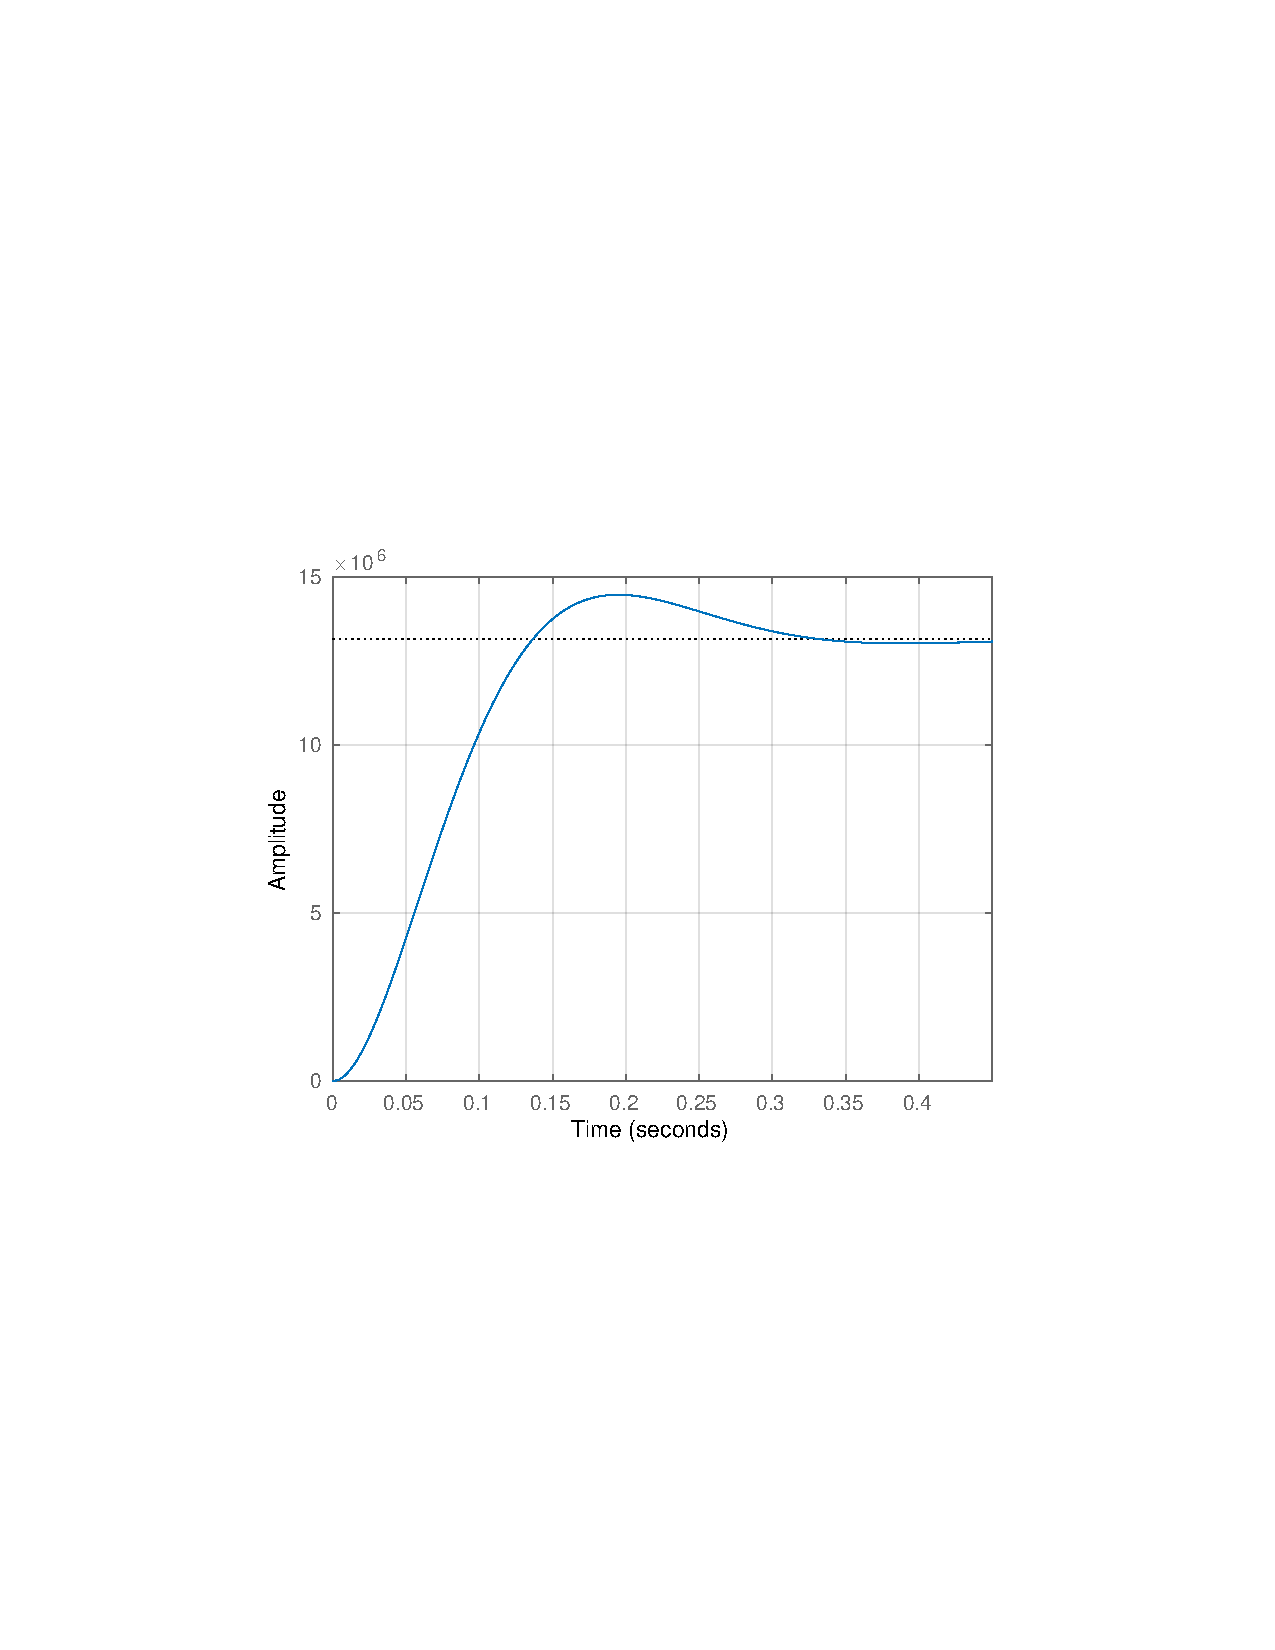
\includegraphics[width=.8\textwidth, trim=100 240 80 252, clip]{5c_step}
	\caption{A rendszer ugrásválasza}
	\label{fig:5c_step}
\end{figure}


%}}}

%{{{ Állandósult érték
\subsection{Állandósult érték}\label{subsec:5d}

Az állapottér rendszerünket írjuk vissza MATLAB segítségével átviteli függvény
alakra ($\fn{W}_\text{cl}$), amivel könnyen tudunk állandósult értéket számolni.
A bemenet legyen $\fn{X} = \frac{\omega_\text{noload}}{s}$, a rendszer válasz $\fn{Y} = \fn{W}_\text{cl}\fn{X}$.

A végérték-tétel alapján az állandósult szögsebesség $\omega_\infty = \lim\limits_{s\rightarrow 0}s\fn{Y} = 2\cdot10^7$.%TODO

%}}}

%{{{ Alapkompenzáció számítása
\subsection{Alapkompenzáció számítása}

Ha nincs statikus alapjelkompenzáció, vagyis $\B{K}_\text{rx}\equiv0$, akkor éljünk
a $\B{K}_\text{ru}:=\B{K}_\text{r}$ jelöléssel, az érthetőség kedvéért.

Most állítsuk be a $\B{K}_\text{r}$ mátrixot úgy, hogy
$\lim\limits_{t\rightarrow\infty}\B{y}=\B{r}$ igaz legyen.
Ezt a következő összefüggés adja meg:

\begin{equation}
	\B{K}_\text{r} = -\brc{\B{C}\widetilde{\B{A}}^{-1}\B{B}}^{-1} = \mat{4,6684\cdot10^{-5}}.
\end{equation}

%}}}

%{{{ Alapjelkompenzált ugrásválasz
\subsection{Alapjelkompenzált ugrásválasz}

\begin{figure}[H]
	\centering
	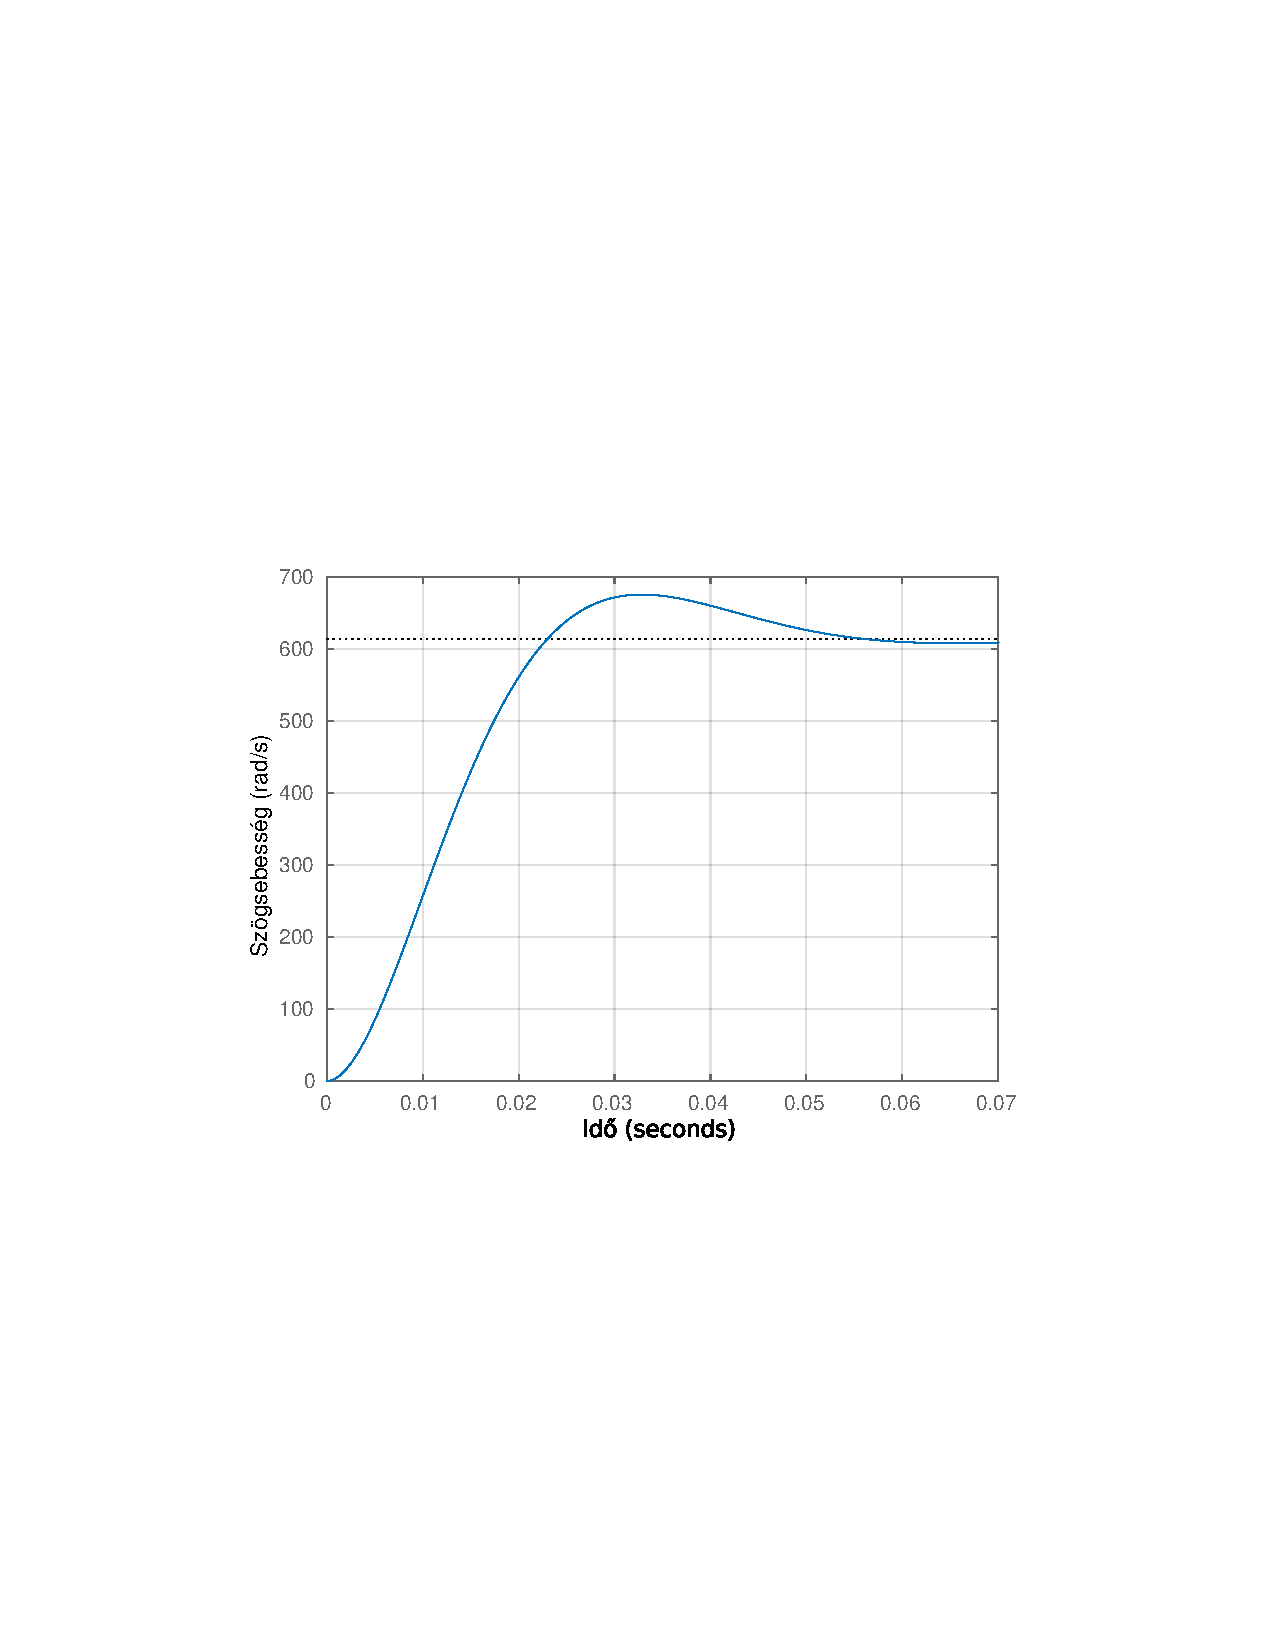
\includegraphics[width=.7\textwidth, trim=100 240 80 252, clip]{5f_step}
	\caption{A rendszer ugrásválasza alapjelkompenzálóval}
	\label{fig:5f_step}
\end{figure}

%}}}

%{{{ Állandósult érték
\subsection{Állandósult érték}

\Aref{subsec:5d}. részfeladathoz hasonló módon járunk el.
A végérték-tétel alapján az állandósult szögsebesség $\omega_\infty = \lim\limits_{s\rightarrow 0}s\fn{Y} = 932,648$.%TODO

%}}}

%{{{ Statikus alapjelkompenzáció
\subsection{Statikus alapjelkompenzáció}

Most legyen $\B{K}_\text{rx}$ nullától különböző.
Ekkor
\begin{equation}
	\mat{\B{K}_\text{rx}\\\B{K}_\text{ru}}=\mat{\B{A}&\B{B}\\\B{C}&\B{D}}^{-1}\mat{\B{0}\\\B{I}}
	= \mat{1,17\cdot10^{-7}\\0\\0,0582}.
\end{equation}

%}}}

%{{{ Statikus alapjelkompenzált ugrásválasz
\subsection{Statikus alapjelkompenzált ugrásválasz}

Írjuk fel a rendszer átviteli függvényét $\B{r}$-től $\B{y}$-ig.
\begin{align}
	\B{u} &= \brc{\B{K}_\text{ru}+\B{K}_\text{x}\B{K}_\text{rx}}\B{r} - \B{K}_\text{x}\B{x}\\
	\B{x} &= \frac{1}{s}\brc{\B{B}\B{u} + \B{A}\B{x}}\\
	\B{x} &= \frac{1}{s}\brc{\B{B}\brc{\B{K}_\text{ru}+\B{K}_\text{x}\B{K}_\text{rx}}\B{r}+\brc{\B{A}-\B{B}\B{K}_\text{x}}\B{x}}\\
	\B{x} &= \brc{\B{I}-\frac{1}{s}\brc{\B{A}-\B{B}\B{K}_\text{x} }}^{-1}\frac{1}{s}\B{B}\brc{\B{K}_\text{ru}+\B{K}_\text{x}\B{K}_\text{rx}}\B{r}\\
	\B{y} &= \B{C}\B{x} = \fbox{$\frac{400}{s^2 + 23,646 s + 400}$}
\end{align}

Az egységugrás válasz ebből a szokásos módon számítható.
\begin{figure}[H]
	\centering
	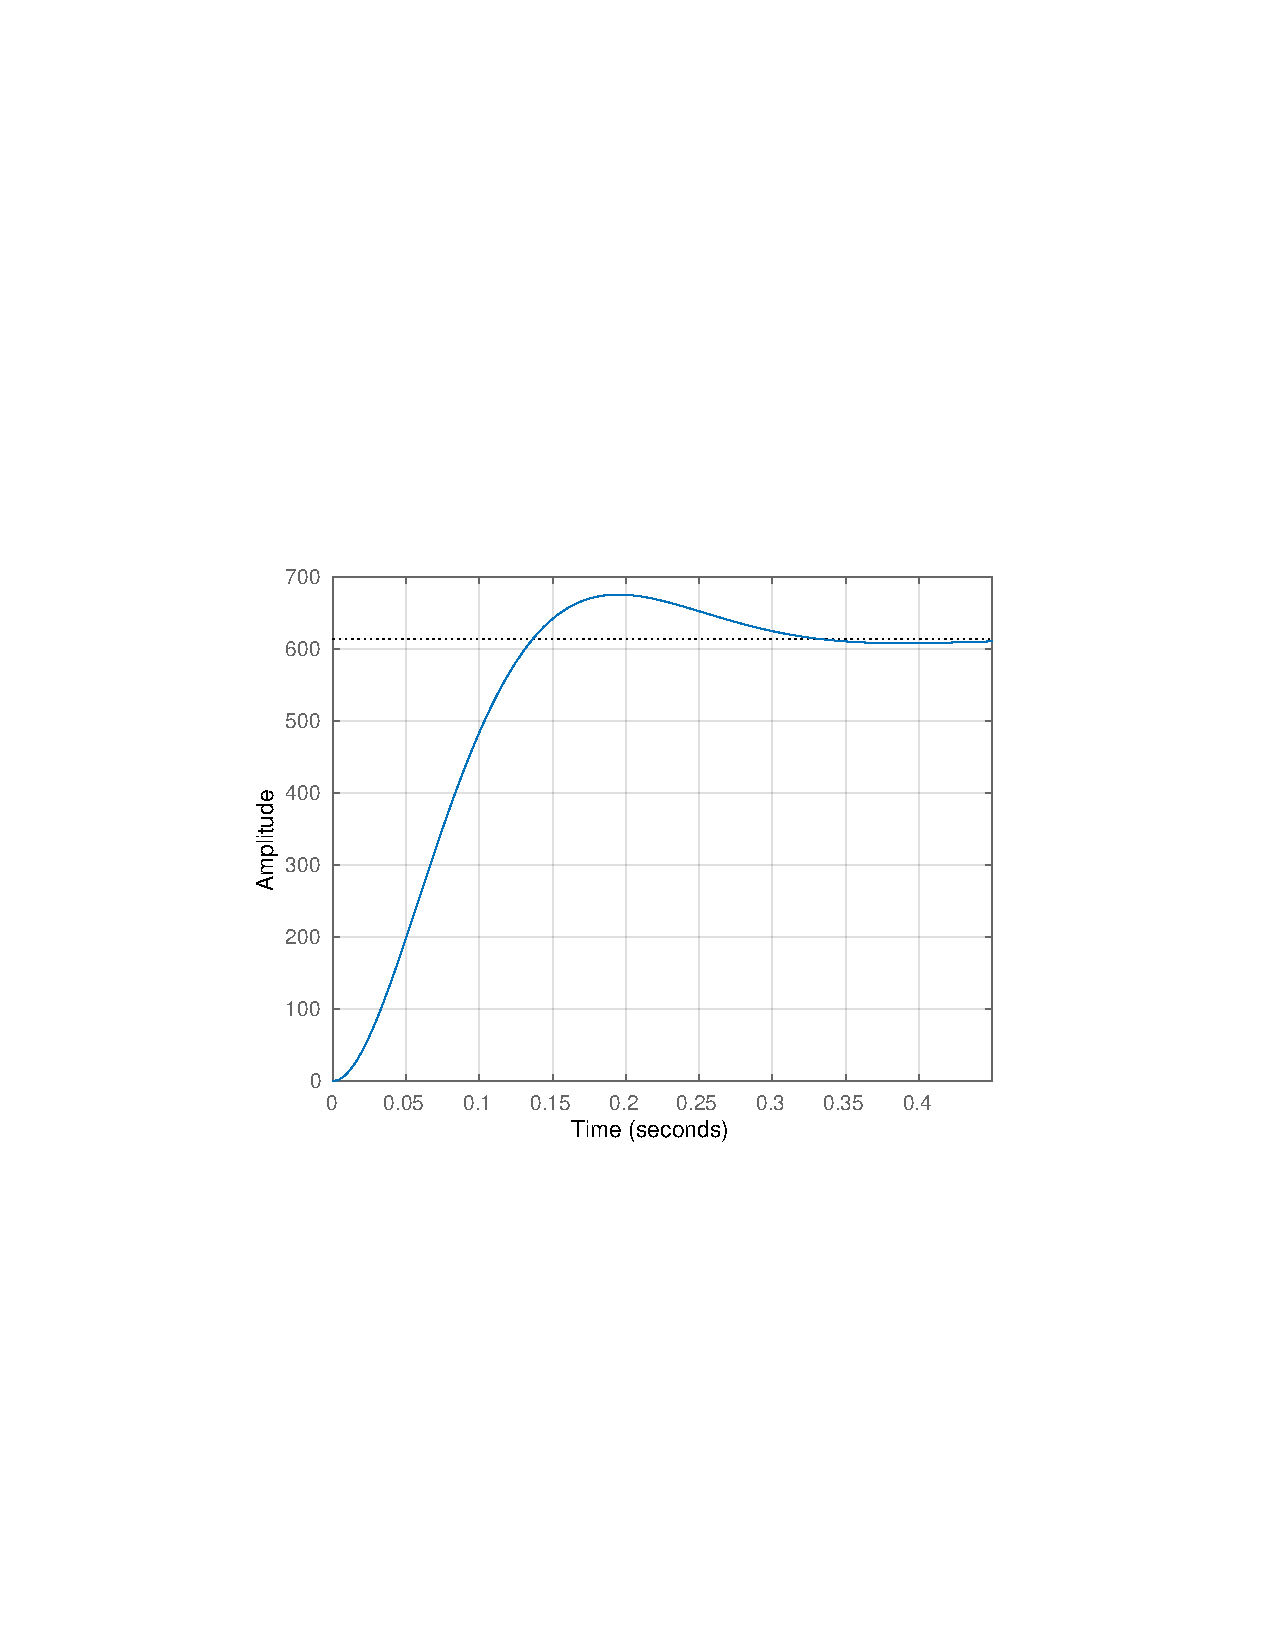
\includegraphics[width=.7\textwidth, trim=100 240 80 252, clip]{5i_step}
	\caption{A rendszer ugrásválasza statikus alapjelkompenzálóval}
	\label{fig:5i_step}
\end{figure}

%}}}

%{{{ Állandósult érték
\subsection{Állandósult érték}

A végérték-tétel alapján az állandósult szögsebesség $\omega_\infty = \lim\limits_{s\rightarrow 0}s\fn{Y} = 932,648$.

%}}}
